\section{Application-level conventions}\label{sec:application_level_conventions}

\subsection{Identifier distribution}

An overview of related concepts is provided in chapter \ref{sec:basic_concepts}.

\subsubsection{Node ID}

Valid values of node ID range from 0 to 127, inclusive.

The node ID values 126 and 127 are reserved for diagnostic and debugging tools;
these node ID values should not be used in fielded systems.

\subsubsection{Port ID}

The subject and service identifier values are segregated into three ranges:
unregulated port identifiers that can be freely chosen by users and integrators (both fixed and non-fixed);
regulated fixed identifiers for non-standard data type definitions
that are assigned by the UAVCAN maintainers for publicly released data types;
and regulated identifiers of the standard data types that are an integral part of the UAVCAN specification.

More information on the subject of data type regulation is provided in section
\ref{sec:basic_concepts_data_type_regulation}.

The ranges are summarized in the table \ref{table:application_port_id_distribution}.
Unused gaps are reserved for future expansion of adjacent ranges.

\begin{UAVCANSimpleTable}{Port identifier distribution}{|l l X|}\label{table:application_port_id_distribution}
    Subject ID          & Service ID        & Purpose \\
    $[0, 32767]$        & $[0, 127]$        & Unregulated identifiers (both fixed and non-fixed). \\
    $[57344, 59391]$    & $[256, 319]$      & Non-standard regulated identifiers (i.e., vendor-specific). \\
    $[62804, 65535]$    & $[384, 511]$      & Standard regulated identifiers. \\
\end{UAVCANSimpleTable}

\subsection{Coordinate frames}

UAVCAN follows the conventions that are widely accepted in relevant applications.
Adherence to the conventions described here maximizes system compatibility and reduces the amount of
computations that would otherwise be required for conversions between incompatible coordinate systems
and representations.
It is recognized, however, that some applications may find the advised conventions unsuitable,
in which case deviations are permitted.
Any such deviations must be explicitly documented.

All coordinate systems are right handed.

\subsubsection{World frame}

For world fixed frames, the \emph{North-East-Down} (NED) right handed notation should be preferred.
It is illustrated on the figure \ref{fig:application_world_frame_convention}.
\begin{samepage}
\begin{description}
    \item[X] --- northward;
    \item[Y] --- eastward;
    \item[Z] --- down.
\end{description}
\end{samepage}

\begin{figure}[hbt]
    \centering
    % The image is released under CC0, public domain, no attribution required:
    % https://commons.wikimedia.org/wiki/File:ECEF_ENU_Longitude_Latitude_relationships.svg
	\includegraphics[width=0.5\textwidth]{application_layer/ECEF_ENU_Longitude_Latitude_relationships}
    \caption{
        World frame convention -- North-East-Down.
        \label{fig:application_world_frame_convention}
    }
\end{figure}

\subsubsection{Body frame}

In relation to a body, the convention is as defined below, right handed.
This convention is widely used in aeronautic applications;
it is illustrated on the figure \ref{fig:application_body_frame_convention}.
\begin{samepage}
\begin{description}
    \item[X] --- forward;
    \item[Y] --- right;
    \item[Z] --- down.
\end{description}
\end{samepage}

\begin{figure}[hbt]
    \centering
    % The source image is released under CC0, public domain, no attribution required:
    % https://pixabay.com/en/airplane-plane-aircraft-propeller-40374/
    % The final image is drawn by me. The source Inkscape SVG file is located in the same directory.
	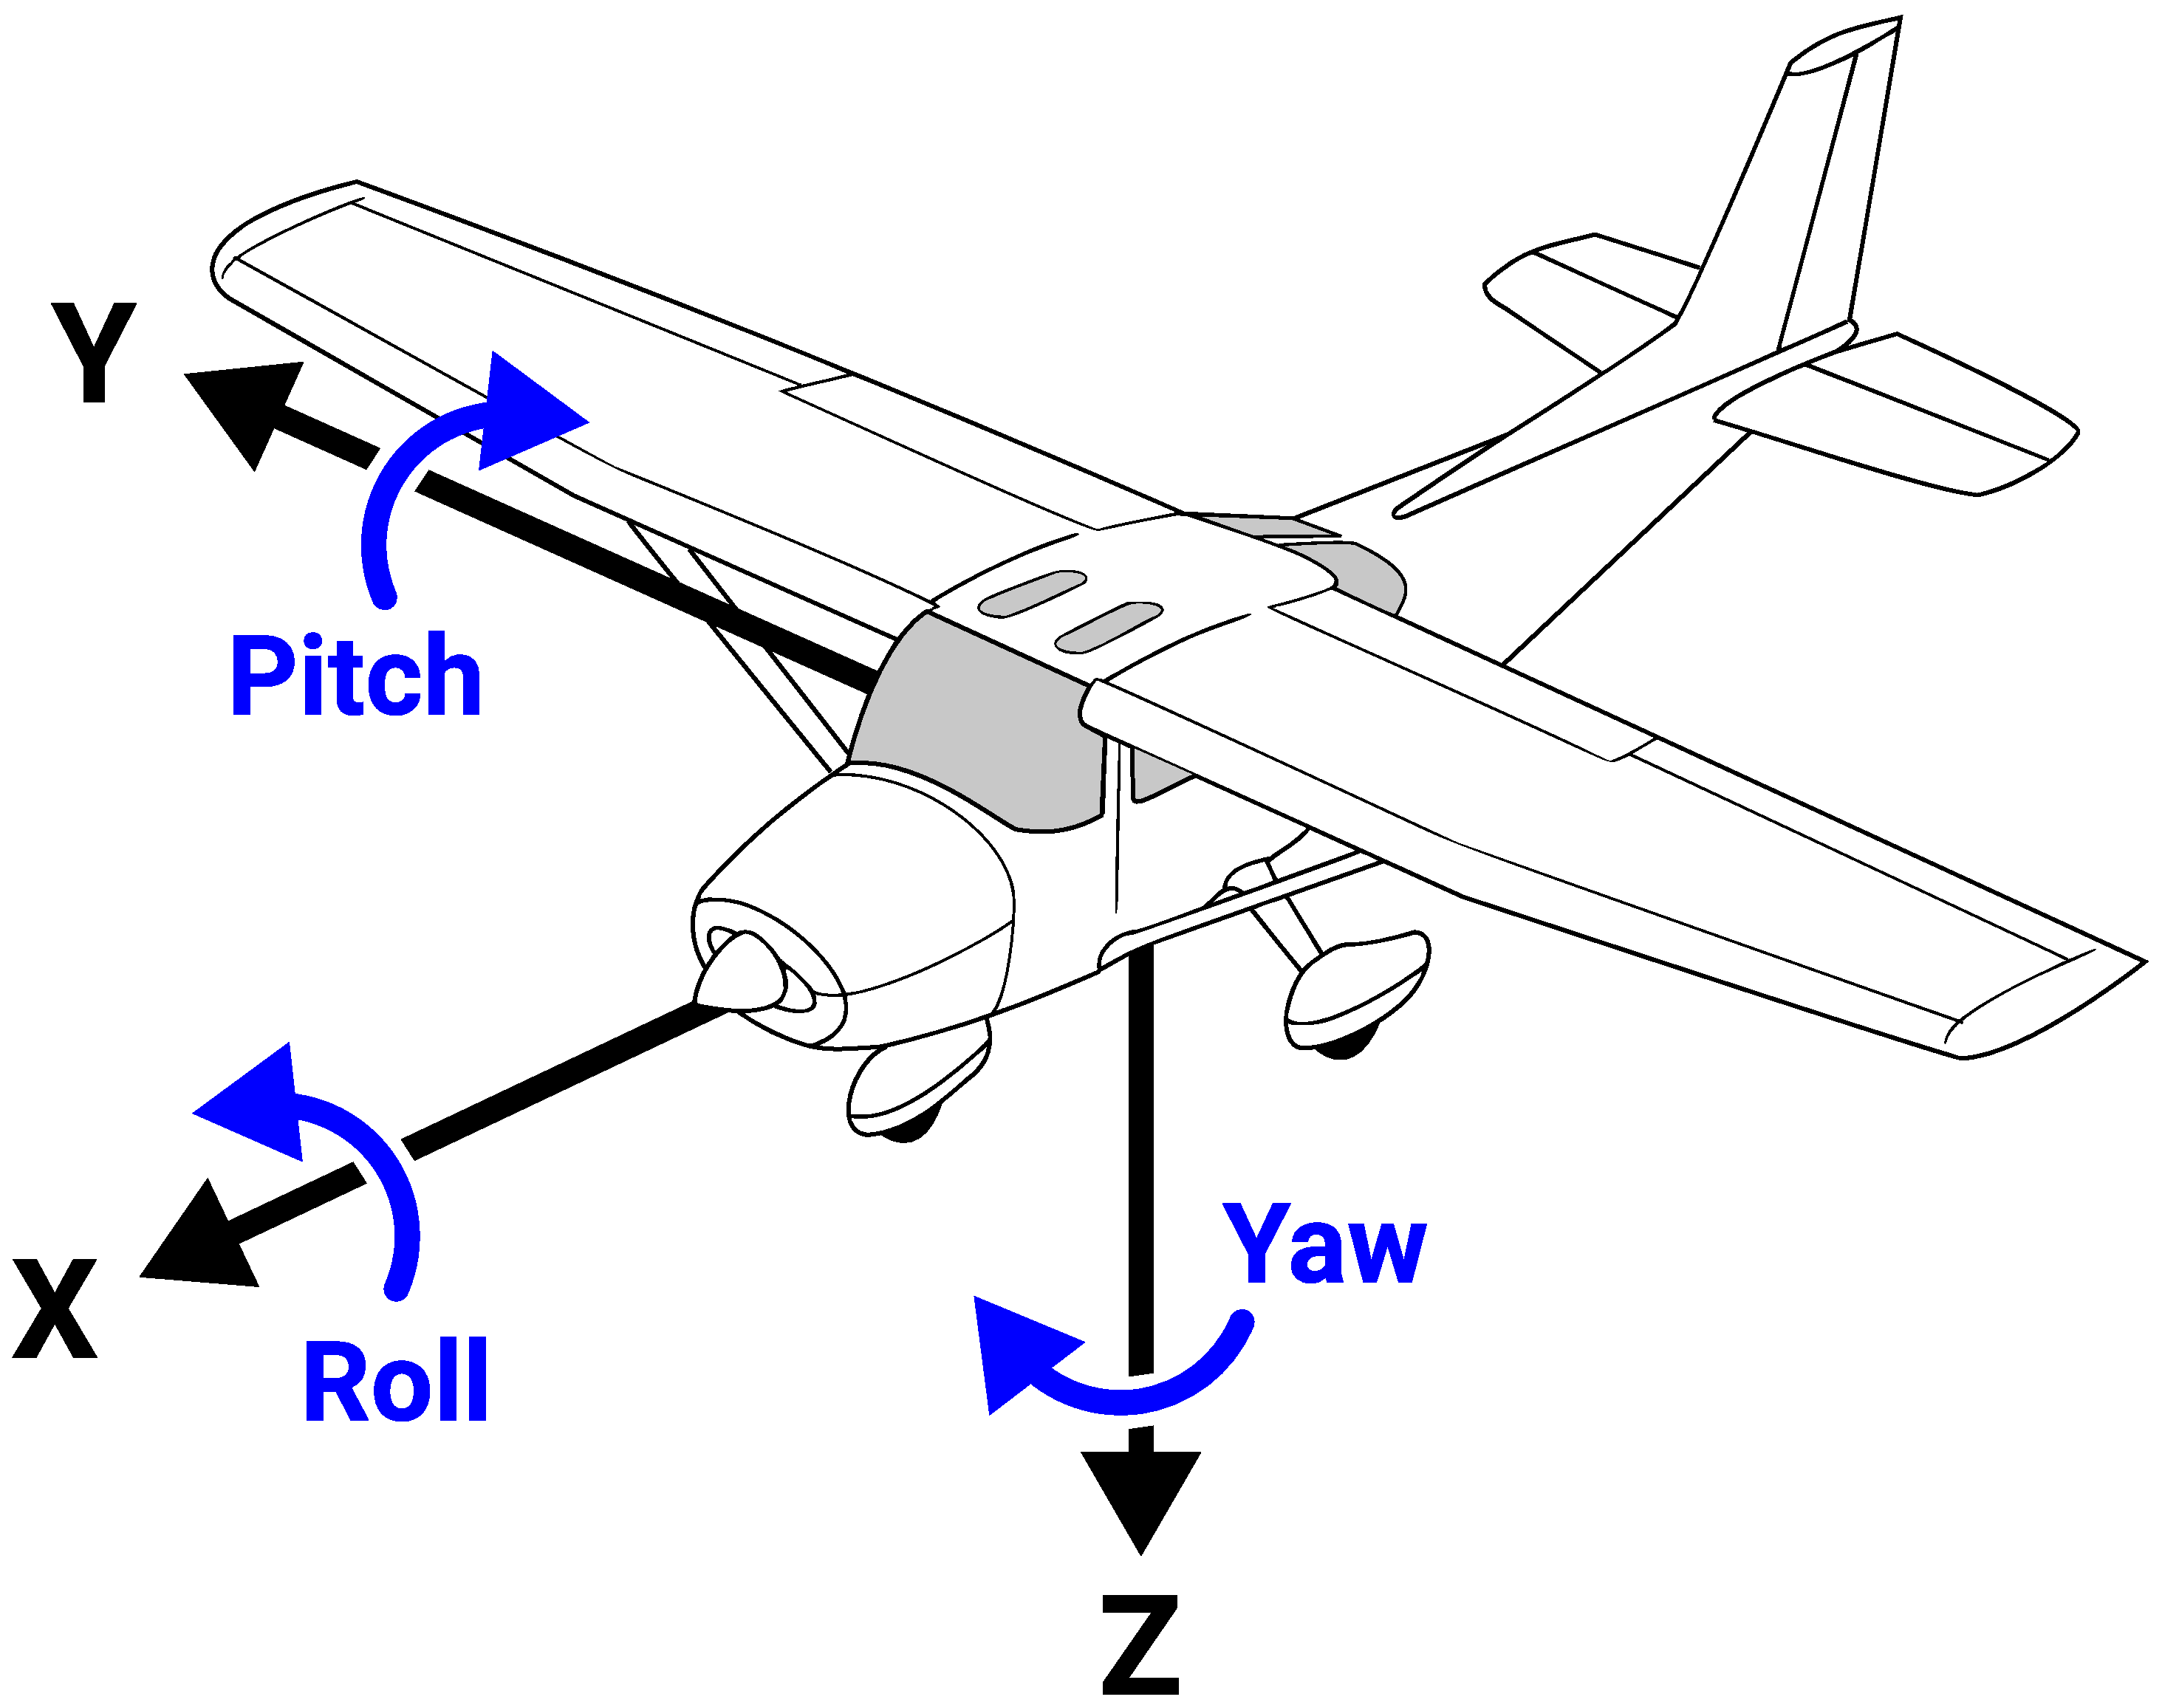
\includegraphics[width=0.5\textwidth]{application_layer/aircraft_principal_axes}
    \caption{
        Body frame convention. Roll, pitch, and yaw arrows indicate positive rotations.
        \label{fig:application_body_frame_convention}
    }
\end{figure}

\subsubsection{Optical frame}

In the case of cameras, the right handed convention specified below should be preferred.
It is widely used in various applications involving computer vision systems.
\begin{samepage}
\begin{description}
    \item[X] --- right;
    \item[Y] --- down.
    \item[Z] --- towards the scene along the optical axis.
\end{description}
\end{samepage}

\subsection{Rotation representation}

\subsection{Matrix representation}

\subsection{Physical quantity representation}
